
\documentclass[10pt,a4paper]{article}
\usepackage[utf8]{inputenc}
\usepackage{amsmath}
\usepackage{amsfonts}
\usepackage{amssymb}
\usepackage{graphicx,subcaption}
\usepackage{listings}
\usepackage[dvipsnames,table,xcdraw]{xcolor}

\usepackage{hyperref}
\hypersetup{
  linktocpage=true,
  colorlinks=true,
  citecolor=Cyan,
  linkcolor=Cyan,
  urlcolor=Magenta       
}

\lstset{frame=tb,
  language=C++,
  aboveskip=3mm,
  belowskip=3mm,
  showstringspaces=false,
  columns=flexible,
  basicstyle={\small\ttfamily},
  numbers=none,
  numberstyle=\tiny\color{Gray},
  keywordstyle=\color{Blue},
  commentstyle=\color{OliveGreen},
  stringstyle=\color{Plum},
  breaklines=true,
  breakatwhitespace=true,
  tabsize=3
}


\title{Binary Search Tree (BST) Traversal Routines}

\begin{document}

\maketitle

\section{Trees}

Graph is another level of abstraction in data structures, built mainly from "Vertices" which are the nodes of the graph and "Edges" which are the pointers connecting the nodes, they are the basic idea behind another structures like trees and binary trees.

Trees are a special case of Graphs, built of the same "vertices" and "edges", changing labels into ("Root","Parent","Child","Leaf"), also trees are sorted in a way that each node have only one parent \cite{bt}\cite{bst}\cite{graph}.

\begin{figure}[htbp]
\centering
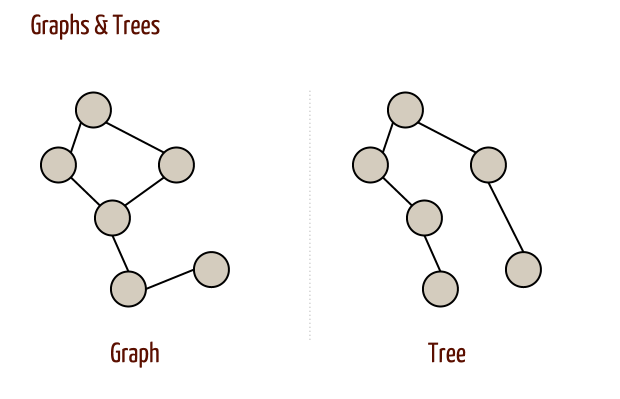
\includegraphics[width=\textwidth]{images/gtree.png}
\caption{\emph{Graphs} vs \emph{Trees}}
\end{figure}


\section{Binary Search Trees}


\begin{figure}[htbp]
\centering
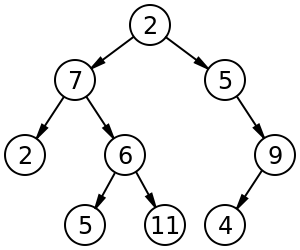
\includegraphics[width=\textwidth]{images/sample_image.png}
\caption{Binary Tree}
\end{figure}

\begin{figure}[htbp]
\centering
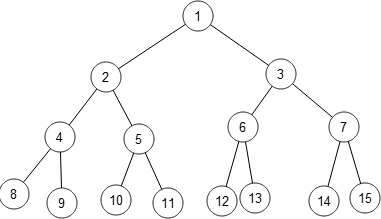
\includegraphics[width=\textwidth]{images/HUufp.png}
\caption{Binary Search Tree}
\end{figure}


As for BST as a special case of BT, BST is actually sorted in an efficent way to help search and retrieve elements in the tree, the way of sorting is conventional, as for the left child is always less than the parent and the right child is always greater.

\subsection{Motivation}

\begin{itemize}
\item As mentioned above, BST is a very efficient way of sorting, searching and retrieving key elements.
\item BST is much more efficient than the array in inserting new nodes, however arrays are better in retrieving.
\item  BST is a sorted linked list, both work just the same, yet BST is more efficient in inserting and retrieving than the linked list due to its earlier sortation.
\end{itemize}

\subsection{Node Structure}

\begin{lstlisting}
struct BSTNode
{
    AnyType data;
    BSTNode *right;
    BSTNode *left;
};
\end{lstlisting}


\subsection{Basic Operations on BST}

\subsubsection{Insertion}


Inserting a node in the tree is a simple process of changing pointers values, as if added from the very bottom -aka leaves- the former leaf has to point at the new leaf, however this process is not the same when adding a node in the middle of the tree, the pointer of the new node itself has to point at the children, and the parent itself has to point at the new node.

\begin{lstlisting}
void insert(BSTNode *&tree, AnyType data)
{   
   
    if (isEmpty(tree))
    {
         root=newnode;
         newnode->right=nullptr;
         newnode->left=nullptr;
    }
    else
    {
        BSTNode *current= new BSTNode;
        current=root;
        while ( current->right!=nullptr || current-left!=nullptr)
            {
                if(current.data>data)
                current=current->right;
                else
                current=current->left;
            }
        if (current->right == nullptr)
        current->right=newnode;
        else
        current->left=newnode;
    }
}

\end{lstlisting}

\emph{Complexity:} $O(n)$

\subsubsection{Removal}

 Removing a node from the BST -it must be a leaf-.

\begin{lstlisting}
    void remove(BSTNode *&tree, AnyType data)
    {
        if(isEmpty(tree))
        break();
        else if (data>current.data)
        current=current->left;
        else
        current=current->right;

        if (isLeaf(current))
        BSTNode *aux= new BSTNode
        //Another loop//
        if (aux->right=current)
        aux->right=nullptr;
        else
        aux->left=null
    }
\end{lstlisting}

\emph{Complexity:} $O(n^2)$

\subsubsection{Traversal}

\begin{itemize}
\item Traversal is the movement in the tree, functions that makes it easier to locate required nodes in certain order, each traversal got its own unique property.
\item Well, for starter, traversing a tree is the easiest way to find required data, trees are sorted already, yet retrieving elements doesn't have to make me start from the very root. 
\end{itemize}
 

\paragraph{In-order}

In-order is a type of traversal that starts from the very left leaf, and ends with the very right leaf, passing through every element in the tree on the way.


\begin{lstlisting}
void inorder(BSTNode *tree)
{
    if (tree)
    {
        while (tree->left!=nullptr)
        {
            tree=tree->left;    //assume we already built a stack

            if(tree->right!=nullptr)
            push(tree->right->data);

            push(tree.data);
        }
        while (tree->right!=nullptr)
        {
            tree=tree->right;

            if(tree->left!=nullptr)
            push(tree->left->data);

            push(tree.data);
        }

    }
        while (top!=nullptr)
        std::cout << "[" << pop(tree.data) << "]";
}
\end{lstlisting}

\emph{Complexity:} $O(n^2)$

\paragraph{Pre-order} 
Pre-order starts from the root, down to the very left leaf, then moves to the right finish all the Left main branch then entering the right main branch and also starting from its very left leaf.

\begin{lstlisting}
void preorder(BSTNode *tree)
{
    //assume there is a pointer pointing at the parent node called *parent//
    if(tree)
    {
        while (current->left!=nullptr)
        {
             current=current->left;
             enqueue(current.data);
        }
        
        while (aux!=root)                      //So illogical, but am building the function as if I know it's size assuming it has only 3 levels//
        {
            aux=aux->parent;
            enqueue(aux->right.data);
            if (aux->right->left!=nullptr)
                enqueue(aux->right->left.data)               //That's so lame I know//
                if (aux->right->right!=nullptr)
                enqueue(aux->right->right.data)  
        }
        while (head!=nullptr)
        std::cout<< "[" << dequeue(tree.data) << "]" ;
    }
}
\end{lstlisting}

\emph{Complexity:} $O(n^2)$

\paragraph{Post-order}
fetching leaves then getting to their parents, efficient way if the required elements are prephiral nodes.

\begin{lstlisting}
void postorder(*tree)
{
    
     while (!isLeaf(tree))
        {
             tree=tree->left;
        }
        enqueue(tree.data);

    if(tree->parent->right!=nullptr)
    enqueue(tree->parent->right.data)
    
    enqueue(parent.data)
    tree=parent
    if(tree->parent->right!=nullptr)
    tree=parent
    while (!isLeaf(tree))
        {
             tree=tree->left;
        }
        enqueue(tree.data)

        if(tree->parent->right!=nullptr)
        enqueue(tree->parent->right.data)

        enqueue(parent.data)
        //doing the same for the main right branch//            //still believe there is a simpler and less stupid algorithm//
}
\end{lstlisting}

\emph{Complexity:} $O(n^2)$


\paragraph{Breadth-first}
It's the simplest way in reading a tree, from top to bottom passing through all the nodes in the way.

\begin{lstlisting}
void BreadthFirst(*tree)
{
    tree=root;
    while(!isLeaf(tree))
    {
    std::cout<< "[" << tree->data << "]" << " " << "[" << tree->left->data << "]" << " " << "[" << tree->right->data << "]" ;
    current=tree;
    tree=tree->left;
    current=current->right;
    std::cout<< "[" << tree->left->data << "]" << " " << "[" << current->left->data << "]" ;
    }

}
\end{lstlisting}

\emph{Complexity:} $O(n^2)$


\bibliographystyle{alpha}
\bibliography{references.bib} 

\end{document}